\section{Consequences of a quasi Riemann hypothesis at $7/8$}\label{pol:sec:qrh}

\subsection{The claim and its status}

On 6 October 2026 OpenAI released a manuscript dated 30 September 2026 \cite{OAI26a}, with a formal proof in Lean, that every Dirichlet $L$ function, $\zeta(s)$ included, has no zeros in the half plane $\re s>\frac78$, and a companion manuscript dated 5 October 2026 \cite{OAI26b} with a separate proof of the weaker half plane $\re s>\frac{11}{12}$. The work has not been refereed; Section~\ref{sec:ch25:open} describes it. Everything in this section is conditional on

\begin{quote}
$(\mathrm Q_{7/8})$\quad $\zeta(s)\ne0$ for $\re s>\frac78$, so that $\sigma_{\max}\le\frac78$ and every zero lies in $\frac18\le\beta\le\frac78$.
\end{quote}

Write $\Delta=\sigma_{\max}-\frac12\le\frac38$ for the half width of the strip containing the zeros of $\Xi$.

\subsection{What moves from $1$ to $7/8$}

\begin{theorem}[Consequences of $\mathrm Q_{7/8}$]\label{pol:thm:qrh}
Assume $(\mathrm Q_{7/8})$.
\begin{enumerate}
\item[(i)] Basepoint laws. For every $\alpha\ge\frac78$ the law $\mu^{(\alpha)}$ with Laplace transform $\xi(\alpha)/\xi(\alpha+\sqrt s)$ is a GGC. For $\alpha>\frac78$ its Thorin measure is absolutely continuous, with density $\pi^{-1}\re\frac{\xi'}{\xi}(\alpha+i\tau)$ in the ordinate variable, a sum of Lorentzians of widths at least $\alpha-\frac78$; it has a stable tail $\mu^{(\alpha)}((y,\infty))\sim b_\alpha/\sqrt{\pi y}$.
\item[(ii)] The clock and Lagarias positivity. For $\alpha>\frac78$ the clock $U_\alpha$ is strictly increasing and $\re\frac{\xi'}{\xi}>0$ on $\re s>\frac78$. In terms of $\zeta$ this is the one sided bound $-\re\frac{\zeta'}{\zeta}(\alpha+i\tau)<\re\mathcal A(\alpha+i\tau)=\frac12\log\frac{\tau}{2\pi}+O(\tau^{-2})$, with $\mathcal A(s)=\frac1s+\frac1{s-1}-\frac12\log\pi+\frac12\frac{\Gamma'}{\Gamma}(\frac s2)$, at every height $\tau$ and for every $\alpha>\frac78$.
\item[(iii)] Even and odd parts. For $\alpha\ge\frac78$ the functions $A_\alpha$ and $B_\alpha$ have only purely imaginary zeros, simple for $\alpha>\frac78$. Proposition~\ref{pol:prop:round}, the exact midpoint formula \eqref{pol:eq:midpoint} and, for $\alpha\le1$, the accounting theorem with $N(\alpha,T)=0$ hold for every $\alpha>\frac78$, and the even part laws $\mu^P_\alpha$ are GGCs there.
\item[(iv)] Heat flow. The de Bruijn Newman constant satisfies $\Lambda\le2\Delta^2\le\frac{9}{32}=0.28125$ by de Bruijn's theorem alone.
\item[(v)] Densities. $N(\sigma,T)=0$ for $\sigma>\frac78$, so in Theorem~\ref{pol:thm:almostall} the exceptional set at a basepoint $\alpha\le\frac78$ is generated only by zeros with $\frac12(\alpha+\frac12)<\beta\le\frac78$.
\end{enumerate}
\end{theorem}

\begin{proof}
(i) By Theorem~\ref{thm:poisson} and Theorem~\ref{rz:thm:threshold}, $\mu^{(\alpha)}$ is a GGC when no zero has real part greater than $\alpha$, and its Thorin measure is the Poisson smoothed zero density, in which a zero of real part $\beta<\alpha$ contributes a Lorentzian of width $\alpha-\beta\ge\alpha-\frac78$; a zero produces an atom only when $\beta=\alpha$, which is why absolute continuity is claimed for $\alpha>\frac78$ only. For the tail, $1-\xi(\alpha)/\xi(\alpha+\sqrt s)\sim b_\alpha\sqrt s$ as $s\downarrow0$, and Karamata's Tauberian theorem for the survival function, with $\Gamma(\frac12)=\sqrt\pi$, gives $\mu^{(\alpha)}((y,\infty))\sim b_\alpha/\sqrt{\pi y}$. (ii) For $\alpha>\sigma_{\max}$ every term $\frac{\alpha-\beta}{|\alpha+i\tau-\rho|^2}$ of the Hadamard sum is positive, so $\re\frac{\xi'}{\xi}(\alpha+i\tau)>0$ and the clock, whose derivative is $\pi^{-1}\re\frac{\xi'}{\xi}(\alpha+i\tau)$, runs forward. Since $\frac{\xi'}{\xi}=\mathcal A+\frac{\zeta'}{\zeta}$, positivity is the stated bound, and $\re\mathcal A(\alpha+i\tau)=\frac12\log\frac\tau{2\pi}+O(\tau^{-2})$ by Stirling's formula for $\frac{\Gamma'}{\Gamma}$. (iii) For $A_\alpha$ this is Theorem~\ref{pol:thm:cosh}(ii) with $\Delta\le\frac38$ and $a=\alpha-\frac12\ge\frac38$. For $B_\alpha$ it is the Hermite Biehler property of $z\mapsto\xi(\alpha-iz)$, which holds whenever $\sigma_{\max}\le\alpha$ (Remark~\ref{pol:rem:easier}; the pairing of $\rho$ with $1-\bar\rho$ proves it). Simplicity follows from the strict monotonicity of the clock in (ii), since the zeros of $A_\alpha(it)$ are transversal crossings of half integer levels. The remaining statements are the propositions cited with $\alpha>\sigma_{\max}$. (iv) In the normalisation $H_0(z)=\frac18\Xi(\frac z2)$ the zeros of $H_0$ lie in $|\im z|\le2\Delta$, and de Bruijn's theorem \cite{deBruijn} makes $H_t$ real rooted for $t\ge\frac12(2\Delta)^2$. (v) is immediate.
\end{proof}

The bound $\Lambda\le\frac{9}{32}$ is weaker than the bound $0.2$ of Platt and Trudgian \cite{PT21}, which sharpens the bound $0.22$ of the Polymath project \cite{Polymath} (Table~\ref{tab:ch21:hist}), obtained by their barrier method and extensive computation; a smaller a priori $\Delta$ might lower those bounds, but that requires redoing the computation. And the stable tails of (i) show what the GGC laws inside the strip look like: the laws at basepoints between $\frac78$ and $1$ have heavy tails of nearly the same weight as the law at $1$, and only the law at $\frac12$ has a finite mean. At the edge the density of (i) can be computed from $\xi$ with no zeros: on $0\le\tau\le60$, $\re\frac{\xi'}{\xi}(\frac78+i\tau)$ is smallest at $\tau=0$, where it equals $\frac{\xi'}{\xi}(\frac78)=0.0173248$, and near each ordinate it has a peak of height at least about $\frac83$ and width $\frac34$, narrower than the smallest gap $1.77$ between ordinates there, so the Thorin measure at $\alpha=\frac78$ already separates the zeros (Figure~\ref{tx5:fig:edge}).

\begin{figure}[t]\centering
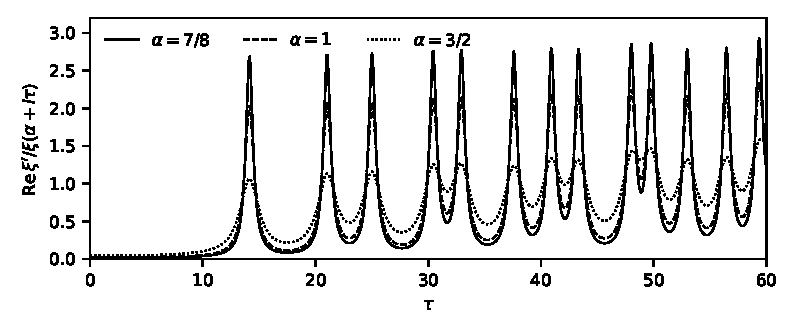
\includegraphics[width=\textwidth]{fig/pol_qrh_edge.pdf}
\caption{The function $\re\frac{\xi'}{\xi}(\alpha+i\tau)$, which is $\pi$ times the Thorin density of Theorem~\ref{pol:thm:qrh}(i) in the ordinate variable, at $\alpha=\frac78$ (solid), $1$ (dashed) and $\frac32$ (dotted) for $0\le\tau\le60$, computed from $\xi$ with no zeros (\texttt{pol\_qrh\_edge.py}). The zeros in this range lie on the critical line, and each contributes a Lorentzian of width $\alpha-\frac12$ and height $1/(\alpha-\frac12)$, that is $\frac83$, $2$ and $1$; at $\alpha=\frac78$ the computed peaks are $2.69$ to $2.93$. On this range the minimum is at $\tau=0$, where the value is $\frac{\xi'}{\xi}(\alpha)=0.0173$, $0.0231$ and $0.0461$. Positivity at every height for $\alpha>\frac78$ is Theorem~\ref{pol:thm:qrh}(ii), under $(\mathrm Q_{7/8})$, and not a consequence of the figure.}\label{tx5:fig:edge}
\end{figure}

Elsewhere in the book the half plane acts as Table~\ref{tx5:tab:map} lists; every entry is conditional on \cite{OAI26a} and is proved where it is cited, except the heuristic count in the last row.

\begin{table}[t]\centering\small
\begin{tabular}{@{}lp{0.78\textwidth}@{}}\toprule
Chapter & What $(\mathrm Q_{7/8})$ gives there\\\midrule
\ref{chap:basepoint} & the compensated L\'evy form for $\frac78<\alpha<1$, with error $O(X^{7/8-\alpha+\delta})$ (Proposition~\ref{bp:prop:below})\\
\ref{chap:strip} & $R(x)=O(x^{7/16+\delta})$ (Theorem~\ref{ri:thm:ggcriesz}); the range $0<y<\frac{4\pi}3$ of Remark~\ref{tx3:rem:qrhrange}\\
\ref{chap:conclusions} & step 7 of the path, with $\alpha=\frac78$ (Section~\ref{sec:ch25:open})\\
\ref{chap:ferro} & $\cosh(at)\,p$ ferromagnetic for $a\ge\frac38$; $\Omega\le\frac38$ (Section~\ref{fm:sec:tilts})\\
\ref{chap:phase}, \ref{chap:tf} & $\Lambda\le\frac9{32}$, weaker than $0.2$ (Corollary~\ref{cp:cor:known})\\
\ref{chap:zhu} & the bound on $\zeta'/\zeta$ behind $v_\alpha>0$ is Theorem~\ref{pol:thm:qrh}(ii) (Section~\ref{zh:sec:comb})\\
\ref{chap:dc} & equivalent to the damped form being nonnegative; $\lambda_{\min}(\frac78,a)\ge0$ (Theorem~\ref{dc:thm:damped})\\
\ref{chap:gl} & with the half plane for every Dirichlet $L$ function, Theorem~\ref{gl:thm:ls} for every $q\ge3$; the heuristic count of Section~\ref{gl:sec:oct} does not lower $K$\\
\bottomrule\end{tabular}
\caption{Where the half plane $\re s>\frac78$ of \cite{OAI26a}, which has not been refereed, acts outside this section.}\label{tx5:tab:map}
\end{table}

\begin{proposition}[Poles of the reciprocal under $\mathrm Q_{7/8}$]\label{tx5:prop:sliver}
Assume $(\mathrm Q_{7/8})$. Every pole $(\rho-\frac12)^2$ of $1/\xi(\frac12+\sqrt w)$ lies in the closed region $(\im w)^2\le4\Delta^2(\Delta^2-\re w)\le\frac9{16}(\frac9{64}-\re w)$, bounded by a parabola with focus $0$ and vertex $\Delta^2\le\frac9{64}$, against the vertex $\frac14$ with no hypothesis. Theorem~\ref{bs:thm:local} holds with the sliver $\mathcal E_{T_0}$ replaced by the thinner set
\[
\mathcal E'_{T_0}=\Bigl\{x+iy:\ x<-T_0^2+\tfrac34T_0+\tfrac9{64},\ y^2\le\tfrac9{16}\bigl(\tfrac9{32}-x\bigr)\Bigr\},
\]
whose half width at the abscissa $-X^2$ is about $\frac34X$, against about $X$ for $\mathcal E_{T_0}$.
\end{proposition}

\begin{proof}
In the notation of the proof of Theorem~\ref{bs:thm:local} a zero is $\gamma=a+ib$ with $0\le b\le\Delta\le\frac38$, and its pole $w=-\gamma^2$ has $\re w=b^2-a^2$ and $(\im w)^2=4a^2b^2=4b^2(b^2-\re w)$, which increases in $b$. In that proof, $b\le\frac38$ in place of $b<\frac12$ gives $x\le2b^2-(a-b)^2<-T_0^2+\frac34T_0+\frac9{64}$ and $y^2\le4b^2(2b^2-x)\le\frac9{16}(\frac9{32}-x)$ on $D_\gamma$, and the rest is unchanged.
\end{proof}

\subsection{The Gaussian smoothed M\"obius sum}\label{tx3:sec:signal}

The proof of \cite{OAI26a} bounds smoothed sums of the M\"obius function twisted by Hecke characters of $\mathbb Q(\sqrt{-3})$ (Section~\ref{sec:ch25:open}), and its last step is a continuation: a bound on the growth of such a sum makes the reciprocal $L$ function analytic in a half plane. Liu \cite{Liu26a} claims an optimisation of its exponents to the half plane $\re s>0.874957\ldots$, and in a second preprint \cite{Liu26b}, the half plane $\re s>B_\flat=0.8748866470\ldots$, with $B_\flat$ the root near $0.8749$ of $133488B^4-376596B^3+384534B^2-167541B+26231$, for every Hecke $L$ function of finite order over every number field $K$, obtained over $K(\zeta_{12})$ and carried down to $K$. Xu and Sang \cite{XuSang26}, assuming the analytic inputs of \cite{OAI26a}, give $8748867/10^7\approx0.8748867$, which agrees with $B_\flat$ to six digits. All of these claims rest on the argument of \cite{OAI26a}; none is refereed, and the Lean proof covers $\frac78$ only. We checked only that $B_\flat$ is a root of the quartic. Nothing below uses them: $B_\flat$ lies $1.13\times10^{-4}$ below $\frac78$ and would change the bound of Theorem~\ref{pol:thm:qrh}(iv) from $0.28125$ to $2(B_\flat-\frac12)^2=0.28108$. For $\zeta$ alone, with a Gaussian weight in the Mellin variable, the sum and its explicit formula can be written down and computed, and nothing in this subsection depends on $(\mathrm Q_{7/8})$. For $x>0$ put
\begin{equation}\label{tx3:eq:signal}
M_{\mathrm g}(x)=\frac1{2\pi i}\int_{(2)}x^{v-2/3}\,\frac{e^{(v-5/6)^2}}{\zeta(v)}\,dv=\frac{x^{-2/3}}{2\sqrt\pi}\sum_{n\ge1}\mu(n)\Big(\frac xn\Big)^{5/6}\exp\Big(-\frac14\log^2\frac xn\Big),
\end{equation}
where the second form follows from $1/\zeta(v)=\sum_n\mu(n)n^{-v}$ and
\[
\frac1{2\pi i}\int_{(c)}e^{vw}e^{(v-c)^2}dv=\frac{e^{cw-w^2/4}}{2\sqrt\pi},
\]
a M\"obius sum smoothed by a Gaussian of standard deviation $\sqrt2$ in $\log n$ around $\log x$.

\begin{proposition}\label{tx3:prop:signal}
Let $\sigma_{\max}=\sup\re\rho$.
\begin{enumerate}
\item[(i)] For every $K\ge1$ there are heights $T_m\in[m,m+1]$ such that for every $x>0$
\[
M_{\mathrm g}(x)=\lim_{m\to\infty}\sum_{|\gamma|<T_m}\operatorname*{Res}_{v=\rho}\frac{x^{v-2/3}e^{(v-5/6)^2}}{\zeta(v)}+\sum_{k=1}^K\frac{e^{(2k+5/6)^2}}{\zeta'(-2k)}\,x^{-2k-2/3}+I_K(x),
\]
with
\[
I_K(x)=\frac1{2\pi i}\int_{(-2K-1)}x^{v-2/3}e^{(v-5/6)^2}\zeta(v)^{-1}dv=O(x^{-2K-5/3}).
\]
At a simple zero the residue is $e^{(\rho-5/6)^2}x^{\rho-2/3}/\zeta'(\rho)$. As $K\to\infty$ the trivial zero series diverges: its $k$th term has modulus
\[
\frac{2(2\pi)^{2k}e^{(2k+5/6)^2}x^{-2k-2/3}}{(2k)!\,\zeta(2k+1)}.
\]
\item[(ii)] $\sigma_{\max}\le\sigma$ if and only if $M_{\mathrm g}(x)=O(x^{\sigma-2/3+\varepsilon})$ as $x\to\infty$ for every $\varepsilon>0$. RH is the exponent $-\frac16$ and $(\mathrm Q_{7/8})$ the exponent $\frac5{24}$.
\item[(iii)] $M_{\mathrm g}(x)=c_1x^{-8/3}+E(x)+O(x^{-11/3})$, with $c_1=e^{(17/6)^2}/\zeta'(-2)=-1.00659\times10^5$ and $E$ the sum over the zeros in (i), and $E(x)$ is not $O(x^{\sigma-2/3})$ for any $\sigma<\sigma_{\max}$. So $c_1x^{-8/3}$ is the leading term of $M_{\mathrm g}$ on a finite range of $x$ only, not its asymptotic.
\end{enumerate}
\end{proposition}

\begin{proof}
(i) Move the line of integration from $\re v=2$ to $\re v=-2K-1$ inside the rectangles $|\im v|<T_m$. On the horizontal sides $|e^{(v-5/6)^2}|=e^{(\re v-5/6)^2-T_m^2}$, and $T_m\in[m,m+1]$ can be chosen with $|\zeta(\sigma\pm iT_m)|^{-1}\le e^{C(\log T_m)^2}$ for $-2K-1\le\sigma\le2$ (\cite[Chapter 9]{Titchmarsh} for $-1\le\sigma\le2$, the functional equation to the left of $-1$), so the horizontal integrals tend to zero. The residues at $v=-2k$ use $\zeta'(-2k)=(-1)^k(2k)!\,\zeta(2k+1)/(2(2\pi)^{2k})$; at $v=1$ the integrand vanishes. (ii) If $M_{\mathrm g}(x)=O(x^{\sigma-2/3+\varepsilon})$, then $\int_0^\infty M_{\mathrm g}(x)x^{2/3-v}\,dx/x$ converges absolutely for $\re v>\sigma+\varepsilon$, since near $x=0$ the series in \eqref{tx3:eq:signal} gives $M_{\mathrm g}(x)x^{2/3}=O(x^{5/6}e^{-\log^2x/4})$. By Mellin inversion it equals $e^{(v-5/6)^2}/\zeta(v)$ for $\re v>1$, hence for $\re v>\sigma+\varepsilon$ by continuation, so $\zeta$ has no zero there. Conversely, if $\sigma_{\max}\le\sigma$, then $1/\zeta(v)=O(|\im v|^{\varepsilon})$ on $\re v\ge\sigma+\varepsilon$, $|\im v|\ge1$, by the Borel and Carath\'eodory argument of \cite[Section 14.2]{Titchmarsh}, which uses only the absence of zeros to the right of $\sigma$; moving the line to $\re v=\sigma+\varepsilon$ gives the bound. (iii) Take $K=1$ in (i). If $E(x)=O(x^{\sigma-2/3})$ with $\sigma<\sigma_{\max}$, then $M_{\mathrm g}(x)=O(x^{\sigma'-2/3})$ with $\sigma'=\max(\sigma,-2)<\sigma_{\max}$, and (ii) gives $\sigma_{\max}\le\sigma'$, a contradiction.
\end{proof}

Computed three ways, from the M\"obius sum over $n\le4\times10^7$ and from the integral on $\re v=2$ and on $\re v=0.6$, between which no zero lies below height $3\times10^{12}$ \cite{PT21}, far beyond the reach of the Gaussian factor, $M_{\mathrm g}(10^3)=-5.53094\times10^{-4}$; the ratio $M_{\mathrm g}(x)/(c_1x^{-8/3})$ is $0.5495$, $0.9470$, $0.99856$ and $0.999983$ at $x=10^3$, $10^4$, $10^5$ and $10^6$ (\texttt{qrh.py}; the M\"obius sum is accurate only while its window $n\lesssim xe^8$ fits below $4\times10^7$). The first pair of zeros has coefficient $|e^{(\rho_1-5/6)^2}/\zeta'(\rho_1)|=2.404\times10^{-87}$ and overtakes $c_1x^{-8/3}$ only at $x\approx10^{36.5}$. Below that the sum is numerically its trivial zero term, and whether its exponent is $-\frac16$ or larger cannot be seen at any computable $x$. The continuation step does not need to see it: it reads the exponent, which the rightmost zero sets however small its coefficient. Since $\sigma_{\max}=\frac12$ is RH, reading an exponent is no obstruction in itself; what stops a method of this kind is the size of the exponents it can prove.


$M_{\mathrm g}$ is the Mellin counterpart of the density $f$ of the clock $T$ (Section~\ref{sec:ch18:law}). Both invert a reciprocal, $e^{(v-5/6)^2}/\zeta(v)$ on a vertical line and $\xi(\frac12)/\xi(\frac12+\sqrt u)$ on a Bromwich line, and both have two expansions. On the prime side each is a M\"obius series with no hypothesis, \eqref{tx3:eq:signal} here and Proposition~\ref{tx3:prop:mobius} there. On the zero side each is a residue series, Proposition~\ref{tx3:prop:signal}(i) here and, under RH with simple zeros, $f(t)=\sum_kR_ke^{-\gamma_k^2t}$ there. They differ in the archimedean factor. The Gaussian is chosen, and it puts the factor $e^{-\gamma^2}$ into the weight of each zero. The clock carries the gamma factor of $\xi$, which puts $e^{-\pi\gamma_k/4}$ into $|\xi'(\rho_k)|$, so that the residues $R_k$ grow like $e^{\pi\gamma_k/4}$ up to powers of $\gamma_k$ and the factor $1/|\zeta'(\rho_k)|$. That is why the spectral expansion of $P(T>t)$ at $t=0.008$ is far off with $20$ zeros and within $10^{-8}$ with $50$ (\texttt{bn\_tail.py}, part b), while $M_{\mathrm g}$ shows no zero below $x=10^{36}$.

\begin{proposition}[Mertens function under $\mathrm Q_{7/8}$]\label{tx5:prop:mertens}
Assume $(\mathrm Q_{7/8})$. Then $M(x)=\sum_{n\le x}\mu(n)=O(x^{7/8+\varepsilon})$ for every $\varepsilon>0$, and $\sum_n\mu(n)n^{-s}$ converges to $1/\zeta(s)$ on $\re s>\frac78$. So the M\"obius series of $1/\zeta(\frac12+\sqrt s)$ converges on $H_{3/8}=\{\re\sqrt s>\frac38\}=\{u+iy:\ u>\frac9{64}-\frac{16}9y^2\}$, which contains the region $H_{1/2}$ of absolute convergence of Section~\ref{ch:rz1}.
\end{proposition}

\begin{proof}
With no zero in $\re s>\frac78$, $\log\zeta$ is analytic there, and the argument of \cite[Section~14.2]{Titchmarsh}, with $\frac78$ in place of $\frac12$, gives $1/\zeta(s)=O(|t|^\varepsilon)$ uniformly on $\re s\ge\frac78+\varepsilon$, $|t|\ge2$. Perron's formula with the contour on $\re s=\frac78+\varepsilon$, as in \cite[Section~14.25]{Titchmarsh}, gives the bound on $M$. Partial summation makes the series converge locally uniformly on $\re s>\frac78$, and its sum, analytic there, equals $1/\zeta$ on $\re s>1$. With $\sqrt s=c+id$, $s=c^2-d^2+2icd$, and $c=\frac38$ traces $x=\frac9{64}-\frac{16}9y^2$.
\end{proof}

This is the unsmoothed form of Proposition~\ref{tx3:prop:signal}(ii), whose exponent $\frac5{24}$ is $\frac78-\frac23$.

\begin{remark}[Least prime in a progression]\label{tx5:rem:leastprime}
Assume, as \cite{OAI26a} claims, that no Dirichlet $L$ function vanishes in $\re s>\frac78$, so that every nontrivial zero has $\frac18\le\beta\le\frac78$ and $|\rho|\ge\frac18$. The explicit formula for $\psi(x,\chi)$ \cite[Chapters~19 and 20]{Davenport} with $T=x$, and $\sum_{|\gamma|\le x}|\rho|^{-1}=O(\log^2(qx))$, give $\psi(x;q,a)=x/\varphi(q)+O(x^{7/8}\log^2(qx))$ uniformly in $(a,q)=1$, so the least prime $p\equiv a\pmod q$ is $O(q^{8+\varepsilon})$ ($7.9928$ with the unrefereed $B_\flat$). This is weaker than the unconditional exponent $5.2$ of Xylouris \cite{Xylouris11}, and it is not the Linnik constant $K$ of Chapter~\ref{chap:gl}.
\end{remark}

\subsection{The compensated clock condition at every height}

\begin{lemma}[Window count]\label{pol:lem:window}
For $d>0$ and $r>d+e$, the number of zeros, counted with multiplicity, with ordinates in $[r-d,r+d]$ is at least
\[
\nu(r,d)=\frac{\vartheta(r+d)-\vartheta(r-d)}{\pi}-s(r+d)-s(r-d),
\]
where $\vartheta$ is the Riemann Siegel theta function, $s(t)=2.5167$ for $e\le t\le X_0=30\,610\,046\,000$, and $s(t)=0.1095\log t+0.2042\log\log t+3.0305$ for $t>X_0$.
\end{lemma}

\begin{proof}
$N(t)=\frac1\pi\vartheta(t)+1+S(t)$ (Section~\ref{sec:ch5:turing}), and $|S(t)|\le s(t)$ for $t\ge e$ by (1.7) and Corollary~1.4 of Hasanalizade, Shen and Wong \cite{HSW22}, as in the proof of Proposition~\ref{bp:prop:v1min}. The bound of Trudgian \cite{Trudgian}, which is often quoted, has an incomplete proof \cite{BMOR21,HSW22} and is not used.
\end{proof}

\begin{theorem}[Compensated clock under $\mathrm Q_{7/8}$, counting form]\label{pol:thm:qrhcomp}
Assume $(\mathrm Q_{7/8})$ and let $\alpha>\frac78$. Put $c_{\min}=\alpha-\frac78$, $c_{\max}=\alpha-\frac18$, $f(c,x)=c/(c^2+x^2)$ and $m(d)=\min\{f(c_{\min},d),f(c_{\max},d)\}$. If for some $d>0$ and some $T_0>d+e$ one has $\nu(r,d)\,m(d)>b_\alpha$ for all $r\ge T_0$, then
\[
D_\alpha(r)=\re\frac{\xi'}{\xi}(\alpha+ir)-\frac{\xi'}{\xi}(\alpha)>0\qquad\text{for all } r\ge T_0 .
\]
For $r+d\le H=3\times10^{12}$ the conclusion also holds if $m(d)$ is replaced by $f(\alpha-\frac12,d)$.
\end{theorem}

\begin{proof}
By the Hadamard product, $D_\alpha(r)=\sum_\rho f(\alpha-\beta_\rho,r-\gamma_\rho)-b_\alpha$, summed symmetrically over all zeros $\rho=\beta_\rho+i\gamma_\rho$ counted with multiplicity. Under $(\mathrm Q_{7/8})$ every width $c_\rho=\alpha-\beta_\rho$ lies in $[c_{\min},c_{\max}]$, because $\frac18\le\beta_\rho\le\frac78$, so every term is positive. For $|r-\gamma_\rho|\le d$ we have $f(c_\rho,r-\gamma_\rho)\ge f(c_\rho,d)$, and $f(\cdot,d)$ increases on $(0,d)$ and decreases on $(d,\infty)$, so its minimum on an interval is attained at an endpoint and $f(c_\rho,d)\ge m(d)$. Lemma~\ref{pol:lem:window} counts the terms, whence $D_\alpha(r)\ge\nu(r,d)\,m(d)-b_\alpha$. For $r+d\le H$ every zero with ordinate in $[r-d,r+d]$ lies on the critical line by the verification of \cite{PT21}, so $c_\rho=\alpha-\frac12$ and $f(c_\rho,d)=f(\alpha-\frac12,d)$.
\end{proof}

Table~\ref{pol:tab:qrh} gives the heights obtained. For each $\alpha$ and each half width $d$ put $k=\lfloor b_\alpha/m(d)\rfloor+1$; if the window holds at least $k$ zeros then $k\,m(d)>b_\alpha$, and by Lemma~\ref{pol:lem:window} it does as soon as $\nu(r,d)\ge k$. The table lists, for the $d$ that makes the last height smallest, the height $T_0$ beyond which $\nu(r,d)\ge k$. Under $(\mathrm Q_{7/8})$ the off line threshold is finite for every $\alpha>\frac78$, because the window count grows like $(\frac d\pi-0.219)\log r$ for $d>0.69$ while $m(d)$ is fixed. For $\alpha$ close to $\frac78$, however, it exceeds the verified height $H$, and then the off line range $r\ge T_0$ and the on line range $r+d\le H$ leave the heights between $H$ and $T_0$ uncovered. The two ranges overlap from $\alpha_*=0.8888$ on: at $\alpha=0.8888$ the count gives $T_0=2.30\times10^{12}$ with $d=3.5$ and sixteen zeros, whereas at $\alpha=0.8887$ it gives $3.19\times10^{12}>H$, and the smallest $\alpha$ for which the off line threshold $T_0$ is at most $H$ is $0.88875$. For the eight basepoints of the table the ranges overlap, and the count covers every height beyond the on line threshold. The scan in $\alpha$ is made by the script on a grid; we do not prove that the thresholds are monotone in $\alpha$, and Theorem~\ref{pol:thm:qrhpair} makes this unnecessary.

\begin{table}[ht]
\centering\small
\fitwidth{\begin{tabular}{cccccc}
\toprule
$\alpha$ & $b_\alpha$ & $T_0$ off line & $(d,k)$ & $T_0$ on line & $(d,k)$\\
\midrule
$0.900$ & $0.01848$ & $1.9\times10^{6}$ & $(3,7)$ & $147$ & $(13,8)$\\
$0.925$ & $0.01963$ & $5.2\times10^{4}$ & $(3.5,5)$ & $147$ & $(13,8)$\\
$0.950$ & $0.02079$ & $1.3\times10^{4}$ & $(5,7)$ & $147$ & $(13,8)$\\
$1.000$ & $0.02310$ & $3.5\times10^{3}$ & $(6.5,8)$ & $147$ & $(13,8)$\\
$1.500$ & $0.04614$ & $324$ & $(8,5)$ & $147$ & $(13,8)$\\
$2.000$ & $0.06907$ & $231$ & $(10.5,7)$ & $147$ & $(13,8)$\\
$5.000$ & $0.20166$ & $191$ & $(12,8)$ & $167$ & $(12.5,8)$\\
$7.800$ & $0.31322$ & $238$ & $(13,10)$ & $214$ & $(12.5,9)$\\
\bottomrule
\end{tabular}}
\caption{Heights beyond which Theorem~\ref{pol:thm:qrhcomp} guarantees the compensated clock inequality under $(\mathrm Q_{7/8})$, rounded up, with the half width $d$ of the window and the number $k$ of zeros that the proof asks for in it. ``Off line'' uses only $\frac18\le\beta\le\frac78$; ``on line'' uses $\beta=\frac12$, valid for $r+d\le H$. Computed by \texttt{polya\_qrh.py} with the bound of Lemma~\ref{pol:lem:window}.}\label{pol:tab:qrh}
\end{table}

The count loses information in one place. A zero at distance $c_{\min}=\alpha-\frac78$ from the line $\re s=\alpha$ contributes only about $c_{\min}/d^2$ to $D_\alpha$, which tends to $0$ with $\alpha-\frac78$, whereas $b_\alpha$ stays near $0.0173$; this is why the method stops at $\alpha_*=0.8888$ rather than at $\frac78$, and why any extension of the verified height only lowers $\alpha_*$ towards $\frac78$.

\begin{theorem}[Compensated clock under a quasi Riemann hypothesis]\label{pol:thm:qrhpair}
Let $\frac12\le\alpha_0<1$ and assume that $\zeta$ has no zero with $\re s>\alpha_0$. Then $D_\alpha(r)>0$ for every $\alpha$ with $\alpha_0<\alpha\le1$ and every real $r\ne0$. Together with Proposition~\ref{bp:prop:valpha}, which has no hypothesis, $D_\alpha(r)>0$ for every $\alpha>\alpha_0$ and every real $r\ne0$.
\end{theorem}

\begin{proof}
Fix $\alpha$ and put $a=\alpha-\frac12$ and $c_{\max}=\alpha+\alpha_0-1$, which is less than $1$ because $\alpha\le1$ and $\alpha_0<1$. As $D_\alpha$ is even we take $r>0$. By the Hadamard product, as in the proof of Theorem~\ref{pol:thm:qrhcomp}, $D_\alpha(r)=\sum_\rho f(\alpha-\beta_\rho,r-\gamma_\rho)-b_\alpha$ with $f(c,x)=c/(c^2+x^2)$. By hypothesis and the functional equation, $1-\alpha_0\le\beta_\rho\le\alpha_0<\alpha$ for every zero, so every width $c_\rho=\alpha-\beta_\rho$ lies in $(0,c_{\max}]$ and every term is positive.

Window estimate. Fix $d>0$ and let $W$ be the multiset of zeros with ordinate in $[r-d,r+d]$, with $n$ elements. The map $\rho\mapsto1-\bar\rho$ preserves the ordinate and the multiplicity and fixes exactly the zeros on the critical line, so $W$ consists of zeros on the line, of width $a$, and of pairs $\{\rho,1-\bar\rho\}$ of the same ordinate whose widths $c,c'$ satisfy $c+c'=2a$ however far from the line the zero lies. For $0<c\le c_{\max}$ and $|x|\le d$ we have $c^2+x^2\le c_{\max}^2+d^2$, hence $f(c,x)\ge c/(c_{\max}^2+d^2)$; summing over $W$, in which the widths add up to $na$,
\[
D_\alpha(r)\ \ge\ \frac{na}{c_{\max}^2+d^2}-b_\alpha\ \ge\ a\Big(\frac{n}{c_{\max}^2+d^2}-0.04621\Big),
\]
by Lemma~\ref{pol:lem:Bbound}. With $d=4$ and $c_{\max}<1$ we have $c_{\max}^2+d^2<17$ and $0.04621\cdot17=0.7856<1$, so $n\ge1$ suffices: if the window $[r-4,r+4]$ contains the ordinate of at least one zero, then $D_\alpha(r)>a\big(\frac1{17}-0.04621\big)>0.0126\,a$.

It remains to show that the window contains an ordinate, or that $D_\alpha(r)>0$ for another reason, at every $r>0$. There are three ranges.

(a) $0<r\le\theta_0=\gamma_1-\alpha/\sqrt3$, where $\theta_0\ge\gamma_1-1/\sqrt3=13.557$. Every zero has $|r-\gamma_\rho|\ge\gamma_1-r\ge\alpha/\sqrt3>c_\rho/\sqrt3$, because $c_\rho<\alpha$, and $x\mapsto f(c,x)$ is strictly convex where $|x|>c/\sqrt3$, since $\partial_x^2f=2c(3x^2-c^2)/(c^2+x^2)^3$. So $D_\alpha$ is strictly convex on $[-\theta_0,\theta_0]$ (the series of second derivatives converges uniformly there), even, and zero at the origin, hence positive for $0<|r|\le\theta_0$; this is the argument of Proposition~\ref{bp:prop:v1min}.

(b) $\theta_0<r\le\gamma_{1700}+4=2201.26$. The first $1700$ ordinates, computed in ball arithmetic and stored in \texttt{data/zeros\_1700.txt}, have consecutive differences at most $6.8873$ (the largest, between $\gamma_1=14.1347$ and $\gamma_2=21.0220$; the next is $5.4140$), so the windows $[\gamma_k-4,\gamma_k+4]$ cover $[\gamma_1-4,\gamma_{1700}+4]$, and $\gamma_1-4=10.13<\theta_0$. Every $r$ of the range lies in one of them, that is, its window contains an ordinate.

(c) $r\ge2200$. By Lemma~\ref{pol:lem:window} with $d=4$ the window holds at least $\nu(r,4)$ zeros, and we show $\nu(r,4)\ge2.42$. Put $I(r)=(\vartheta(r+4)-\vartheta(r-4))/\pi$. Since $\vartheta''(t)=\frac14\sum_{n\ge0}(n+\frac14)t\,\big((n+\frac14)^2+\frac{t^2}4\big)^{-2}>0$, $I$ increases, and on $[2200,X_0-4]$ we have $\nu(r,4)=I(r)-2\cdot2.5167\ge\nu(2200,4)=7.4591-5.0334=2.4257$. For $r\ge X_0-4$ Stirling's formula gives $I(r)=\frac4\pi\log\frac r{2\pi}+O(r^{-2})$ with an error below $10^{-9}$, and $s$ is nondecreasing and, at $t=r+4\ge X_0$, at most $s_{\log}(t)=0.1095\log t+0.2042\log\log t+3.0305$, so $\nu(r,4)\ge\frac4\pi\log\frac r{2\pi}-2s_{\log}(r+4)-10^{-9}$. The derivative of the right side is at least $\big(\frac4\pi-2\cdot0.1095-\frac{2\cdot0.2042}{\log X_0}\big)/(r+4)>1/(r+4)$, so it increases, and at $r=X_0-4$ it equals $28.4018-12.6490-10^{-9}>15.75$. Hence $\nu(r,4)\ge2.42>0$ for all $r\ge2200$, and the window contains a zero. Ranges (b) and (c) overlap in $[2200,2201.26]$.
\end{proof}

For $\alpha_0=\frac12$ the theorem is the direction RH $\Rightarrow$ compensated positivity of Theorem~\ref{thm:dbeta:minall}(vi), and the window argument is that of the proof of part (v) of Theorem~\ref{thm:dbeta:minall}.

\begin{corollary}\label{pol:cor:equiv}
For $\frac12\le\alpha_0<1$ the following are equivalent: (a) $\zeta$ has no zero with $\re s>\alpha_0$; (b) $D_\alpha(r)\ge0$ for every $\alpha\in(\alpha_0,1)$ and every real $r$ at which $D_\alpha$ is defined. When they hold, $D_\alpha(r)>0$ for every $\alpha\in(\alpha_0,1)$ and every real $r\ne0$.
\end{corollary}

\begin{proof}
(a) implies (b) by Theorem~\ref{pol:thm:qrhpair}, and (b) implies (a) by Proposition~\ref{pol:prop:comp}, since $D_\alpha\ge0$ for $\alpha\ge1$ by Proposition~\ref{bp:prop:valpha}.
\end{proof}

For $\alpha_0=\frac12$ this is part (vi) of Theorem~\ref{thm:dbeta:minall}.

\begin{corollary}\label{pol:cor:qrhggc}
Assume $(\mathrm Q_{7/8})$ and let $\alpha>\frac78$. Then the compensated reciprocal $e^{wb_\alpha}\xi(\alpha)/\xi(\alpha+w)$ is the Laplace transform in $u=w^2/2$ of a GGC, with the Thorin density \eqref{pol:eq:stieltjes} of the $2\sin^2$ lemma, positive at every height. For $\alpha\ge1$ this holds with no hypothesis, by the factorisation of Proposition~\ref{bp:prop:valpha}.
\end{corollary}

\begin{proof}
The hypotheses of Theorem~\ref{pol:thm:exactlemma} hold for $\xi$ with $\delta=\alpha-\frac78$, and its condition \eqref{pol:eq:exactlemma} is $D_\alpha\ge0$, which holds by Theorem~\ref{pol:thm:qrhpair} for $\frac78<\alpha\le1$ and by Proposition~\ref{bp:prop:valpha} for $\alpha\ge1$.
\end{proof}

So under the claimed theorem the conclusion of the $2\sin^2$ lemma, positivity of the Thorin density of the compensated reciprocal, holds on every line to the right of $\frac78$, inside the critical strip for $\frac78<\alpha<1$, even though the hypothesis of the lemma, positivity of the primal measure, cannot even be stated there, because the Euler product diverges.

\paragraph{Numerics.} The script \texttt{polya\_qrhpair.py} (\texttt{code/\allowbreak README.md}) computes the constants of the proof of Theorem~\ref{pol:thm:qrhpair} for $\alpha_0=\frac78$ and writes them to \texttt{data/polya\_qrhpair.json}. The margin $a/(c_{\max}^2+16)-b_\alpha$ for one zero in the window, with $b_\alpha$ computed by mpmath at sixty values of $\alpha$ in $(\frac78,1]$, is at least $0.0053$, with the minimum at $\alpha=0.8751$, and the ratio $b_\alpha/a$ is at most $0.04620$; the inequality $f(c,x)+f(2a-c,x)\ge2a/(c_{\max}^2+d^2)$ for a pair holds on grids of $\alpha$, $c$ and $x$ with smallest ratio $1.0000047$. The quantity $\nu(r,4)$ was recomputed with the Stirling series for $\vartheta$ and with mpmath at ten heights up to $10^{16}$, agreeing to $7.1\times10^{-15}$; it never exceeds the number of ordinates in $[r-4,r+4]$ for $r$ from $40$ to $2190$.

The direct computation of $D_\alpha$ agrees. The script \texttt{polya\_primes.py} finds $D_\alpha(r)>0$ on $(0,600]$ at step $0.01$ (60\,000 heights) at $\alpha=0.9$, $0.95$, $1$, $1.001$, $2$, $4$ and $7.8$, and on $(0,200]$ at the fifteen equally spaced basepoints from $1$ to $7.8$ and at twelve further ones ($1.001$, $1.01$, $1.1$, $1.2$, $1.5$, $2$, $3$, $4$, $5$, $6$, $7$ and $7.789$), with the smallest value of $D_\alpha$ at the first height of the grid, where $D_\alpha$ grows like $r^2$ and $D_\alpha(r)/r^2$ is $1.1\times10^{-4}$ at $\alpha=1$ and $9.0\times10^{-4}$ at $\alpha=7.8$. At heights above $2$ the minimum over $(2,600]$ is $3.7\times10^{-4}$, $4.2\times10^{-4}$ and $4.6\times10^{-4}$ at $\alpha=0.9$, $0.95$ and $1$, attained just above $r=2$. These computations use no hypothesis on the zeros, and for $\alpha<1$ they are floating point evidence, not a proof.

\subsection{What it does not give, and what to look for in the proof}

The claimed theorem is a fixed half plane. The routes of this chapter and of the book need more.
\begin{enumerate}
\item Bondesson's closure gives RH from GGC basepoint laws along a sequence $\alpha_n\downarrow\frac12$ (Corollary~\ref{cor:weak:closure}). $(\mathrm Q_{7/8})$ supplies them for $\alpha\ge\frac78$ only; the open strip is $\frac12<\alpha<\frac78$.
\item The even part laws and the accounting theorem need no zero to the right of $\alpha$; below $\frac78$ the term $2N(\alpha,T)$ of Theorem~\ref{pol:thm:accounting} remains and is controlled only by density estimates.
\end{enumerate}

The structural point is Corollary~\ref{pol:cor:equiv}: a quasi Riemann hypothesis at $\alpha_0$ is equivalent to the positivity of the compensated Thorin densities of the $2\sin^2$ lemma on every line to the right of $\alpha_0$. The proof announced in \cite{OAI26a} does not go through the Thorin picture (Section~\ref{sec:ch25:open}), but the equivalence says that whatever it proves has a Thorin reading. If it contains an explicit lower bound for $\re\frac{\zeta'}{\zeta}$ or for a mollified Dirichlet polynomial on $\re s>\frac78$, then a bound at least as strong as $-\re\mathcal A$ is, by part (ii) of Theorem~\ref{pol:thm:qrh}, positivity of the clock, a Thorin statement in disguise, and the natural next step towards $\alpha_0<\frac78$ is to transfer it directly to the clock: the identity \eqref{pol:eq:primes} at $\alpha<1$, with the prime sum replaced by whatever the proof controls.
